\documentclass[a3paper]{article}
\usepackage[a4paper]{geometry}
\usepackage[dvipsnames]{xcolor}
\usepackage{tikz}
\usepackage{verbatim}

\usetikzlibrary{arrows,positioning} 
\tikzset{
    %Define standard arrow tip
    >=stealth',
    %Define style for boxes
    punkt/.style={
           rectangle,
           rounded corners,
           draw=black,
           text width=7cm,
           minimum height=2em,
		   font=\large
	},
	punktc/.style={
           rectangle,
           rounded corners,
           draw=black,
           text width=6cm,
           minimum height=2em,
		   text centered,
		   font=\large
	},
    % Define arrow style
    pil/.style={
           ->,
           thick,
           shorten <=2pt,
           shorten >=2pt,}
}

\begin{document}

\pagestyle{empty}

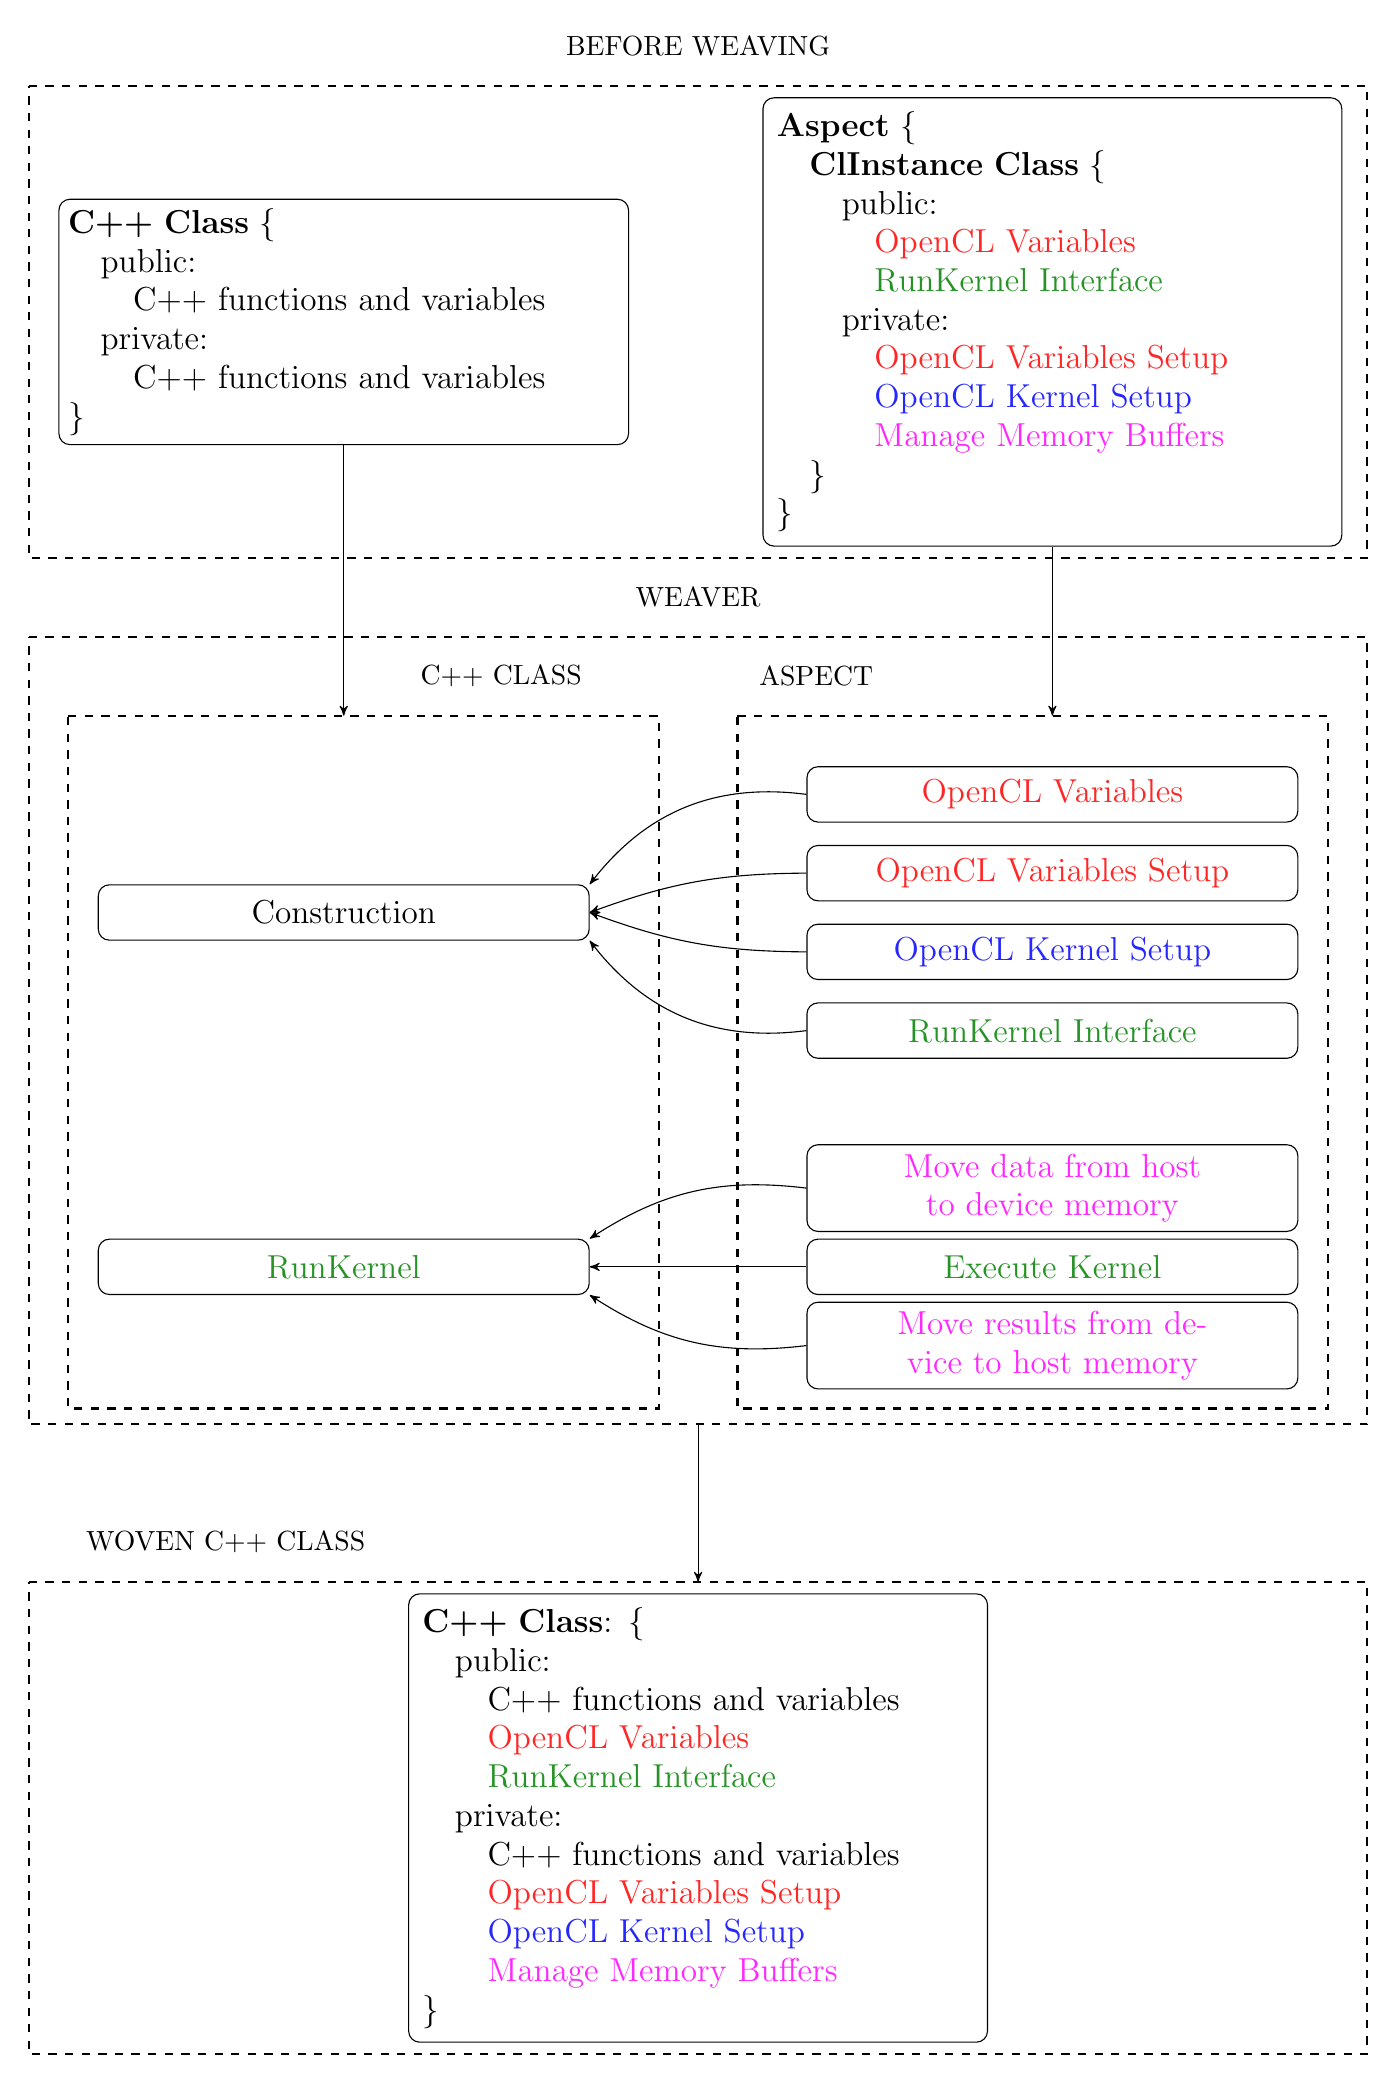
\begin{tikzpicture}[node distance=1cm, auto,]
 %nodes
	\node[punkt] (cppbw) at (3,2){ \textbf{C++ Class} \{			\\
	 \quad public:												\\
	 \qquad  C++ functions and variables						\\
	 \quad private:												\\
	 \qquad  C++ functions and variables						\\
 \}
};

 \node[punkt, inner sep=5pt]
 (aspbw) at (12, 2) { \textbf{Aspect} \{											\\
		 \quad \textbf{ClInstance Class} \{								\\
			\qquad public:												\\
			\quad \qquad \textcolor{Red!85}{OpenCL Variables}			\\
			\quad \qquad \textcolor{Green!85}{RunKernel Interface}		\\
			\qquad private:												\\
			\quad \qquad \textcolor{Red!85}{OpenCL Variables Setup}		\\
			\quad \qquad \textcolor{Blue!85}{OpenCL Kernel Setup}			\\
			\quad \qquad \textcolor{Magenta!85}{Manage Memory Buffers}		\\
			\quad \}															\\
 \}
};

\node[punktc] (const) at (3, -5.5)  { Construction};
\node[punktc] (clvar) at (12, -4) { \textcolor{Red!85}{OpenCL Variables} };
\node[punktc] (clset) at (12, -5) { \textcolor{Red!85}{OpenCL Variables
									Setup} };
\node[punktc] (clker) at (12, -6) { \textcolor{Blue!85}{OpenCL Kernel
									Setup} };
\node[punktc] (clrun) at (12, -7) { \textcolor{Green!85}{RunKernel
									Interface} };

\node[punktc] (crun) at (3, -10)  { \textcolor{Green!85}{RunKernel}};
\node[punktc] (clmem1) at (12, -9)  { \textcolor{Magenta!85}{Move data from host to
	device memory}};
	\node[punktc] (clexec) at (12, -10)  { \textcolor{Green!85}{Execute Kernel}};
	\node[punktc] (clmem2) at (12, -11)  { \textcolor{Magenta!85}{Move results
	from device to host memory}};

 \node[punkt, inner sep=5pt]
 (woven) at (7.5, -17) { \textbf{C++ Class}: \{						\\
			\quad public:												\\
			\qquad C++ functions and variables						\\
			\qquad \textcolor{Red!85}{OpenCL Variables}			\\
			\qquad \textcolor{Green!85}{RunKernel Interface}		\\
			\quad private:												\\
			\qquad C++ functions and variables						\\
			\qquad \textcolor{Red!85}{OpenCL Variables Setup}		\\
			\qquad \textcolor{Blue!85}{OpenCL Kernel Setup}			\\
			\qquad \textcolor{Magenta!85}{Manage Memory Buffers}		\\
 \}
};

\node (name) at (7.5, -1.5) { WEAVER };
\node (name) at (5, -2.5) { C++ CLASS };
\node (name) at (9, -2.5) { ASPECT };
\node (nam1) at (7.5, 5.5) { BEFORE WEAVING };
\node (nam2) at (1.5, -13.5) { WOVEN C++ CLASS};

 % Dots for weaver
\draw[dashed, thick] (-1, -2) -- (16, -2) -- (16, -12) -- (-1, -12) -- (-1, -2);
\draw[dashed, thick] (-1, 5) -- (16, 5) -- (16, -1) -- (-1, -1) -- (-1, 5);
\draw[dashed, thick] (-1, -14) -- (16, -14) -- (16, -20) -- (-1, -20) --
(-1, -14);
\draw[dashed, thick] (-0.5, -3) -- (7, -3) -- (7, -11.8) -- (-0.5, -11.8) --
(-0.5, -3);
\draw[dashed, thick] (8, -3) -- (15.5, -3) -- (15.5, -11.8) -- (8, -11.8) --
(8, -3);

\draw[->] (cppbw.south) -- (3, -3);
\draw[->] (aspbw.south) -- (12, -3);
\draw[->] (7.5, -12) -- (7.5, -14);
\draw[->] (clvar.west) to[bend right=30] (const.north east);
\draw[->] (clset.west) to[bend right=10] (const.east);
\draw[->] (clker.west) to[bend left=10] (const.east);
\draw[->] (clrun.west) to[bend left=30] (const.south east);

\draw[->] (clmem1.west) to[bend right=20] (crun.north east);
\draw[->] (clexec.west) to[bend left=0] (crun.east);
\draw[->] (clmem2.west) to[bend left=20] (crun.south east);

\end{tikzpicture}

\end{document}
